% Provenance (never printed): see sources/outline_sources.md (Year 3: elastic waves
% recalled from the physics books; rays in a spherical Earth; travel-time tables;
% surface waves and dispersion; normal modes, told; linear inverse problems and
% seismic tomography). Brief: sources/book5/BRIEFS.md, ch. 1. Curves from
% figdata/bachelor-3/ray_tracing.py, love_dispersion.py, tomo_checkerboard.py;
% exercise and problem values in the Book 5 scratch calculator calc/ch01.py.
\chapter{علم الزلازل والتصوير الأرضي}\label{ch:b3:seismology-imaging}

في 22 مايو 1960، عند الساعة 19:11 بالتوقيت العالمي، كسر أكبرُ زلزال سُجّل منذ
1900، منطقةَ الاندساس قبالة جنوب تشيلي، بمقدار 9.5.
% ledger: usgs5:chile1960
وصلت موجات P إلى محطات في الجانب البعيد من الكوكب بعد نحو عشرين
دقيقة؛ وطافت موجاتها السطحية حول الكرة الأرضية عدّة مرات؛ ولأيام
بعدها سجّلت أبطأ الأجهزة الأرضَ كلّها تهتزّ
بدورات قريبة من ساعة، كجرسٍ مضروب. وتحمل كلّ من هذه الإشارات
معلومات عن الصخور التي عبرتها. ومن أزمنة وصول ملايين من
موجةٍ، تُقرأ في آلاف المحطات، بنى الزلزاليون لا النموذجَ
الطبقيّ للأرض المذكورَ أدناه فحسب، بل صورًا ثلاثية الأبعاد للوشاح،
تظهر فيها الألواحُ المندسّة والأعمدةُ الصاعدة مناطقَ
تسير فيها الموجات أسرع قليلًا أو أبطأ من المتوسط. يبيّن هذا الفصل كيف:
تنتقل الأشعّة في أرض كروية، وكيف تسبر الموجات السطحية القشرةَ
والوشاحَ عبر تشتّتها، وكيف تُوصف الذبذبات الحرّة للكوكب بأكمله،
وكيف تتحوّل بضعة آلاف من أزمنة الانتقال إلى
صورةٍ بحلّ مسألة عكسية خطية.

\begin{recall}
في جسم صلب مرن متماثل الخواص تنتقل نوعان من الموجات الجسمية: موجات P،
بسرعة $\alpha = \sqrt{(K + \tfrac43\mu)/\rho}$، وموجات S بسرعة
$\beta = \sqrt{\mu/\rho}$، حيث $K$ و$\mu$ معاملا الحجم والقصّ
و$\rho$ الكثافة؛ لا تعبر موجات S السائلَ (من كتب الفيزياء، مجلد السنة الثالثة،
في الفصل المتعلّق بمرونة الأوساط المتصلة). تُسمّى الموجة التي تتوقف سرعتها الطورية
على ترددها موجةً مشتّتة؛ وتنتقل طاقتها بسرعة الزمرة
$U = \mathrm d\omega/\mathrm dk$ (من كتب الفيزياء، مجلد السنة الثانية، في
الموجات). يهتزّ جسم مرن محدود اهتزازًا حرًّا وفق مجموعة منفصلة من الأنماط
العادية (المجلد نفسه). المسافة الإبيسنترية $\Delta$ لمحطة هي الزاوية
عند مركز الأرض بين الإبيسنتر والمحطة؛ ويعطي منحنى زمن الانتقال
زمنَ الوصول الأول بدلالة $\Delta$، وتُحدث النواةُ
منطقةَ ظلّ لموجات P المباشرة (الكتاب 2، الصف 11). والنموذجُ المرجعيّ للأرض،
والانقطاعاتُ الزلزالية وموجةُ الرأس، قد عُرضت في مجلد السنة الأولى،
في فصله عن الأرض الطبقية. وتنتمي المربعات الصغرى وقانون الأخطاء الغوسي
إلى كتب الرياضيات.
\end{recall}

\section{الأشعّة في أرض كروية}

تُتبَع جبهةُ الموجة الزلزالية، بعيدًا عن مصدرها وفي وسط تتغيّر خواصه
ببطء على مدى طول موجة، بأشعّتها: وهي المنحنيات
العمودية في كل مكان على جبهة الموجة، والتي تنتقل عليها الطاقة. وفي وسط
ذي سرعة منتظمة تكون الأشعّة مستقيمة؛ وحيث تتغيّر السرعة تنحني
بحسب قانون سنل للانكسار. وفي الأرض تتعلّق السرعات أساسًا بالعمق،
ولذلك يكون النموذج الأول متماثلًا كرويًّا: السرعة $v(r)$ للموجة
المدروسة (P أو S) دالةٌ لنصف القطر $r$ وحده.

\begin{theorem}[قانون سنل في أرض كروية]\label{thm:b3:seismology-imaging:snell}
في أرض متماثلة كرويًّا ذات سرعة موجية $v(r)$، ليكن $i$ الزاوية
بين شعاعٍ ونصف القطر عند النقطة التي نصف قطرها $r$. على طول الشعاع كلّه،
\[
  \frac{r\sin i}{v(r)} = p
\]
يبقى ثابتًا.
\end{theorem}

\begin{proof}
نستبدل الأرضَ بقشور رقيقة متمركزة، لكلٍّ منها سرعة منتظمة. داخل قشرة
يكون الشعاعُ خطًّا مستقيمًا؛ والخط المستقيم على البعد $d$ من
المركز يلتقي بالكرة ذات نصف القطر $r$ بزاوية $i$ حيث
$r\sin i = d$ (المثلث القائم الذي يكوّنه المركز وقدم العمود
والنقطة)، فيكون $r\sin i$ هو نفسه عند أعلى القشرة وعند أسفلها. وعند الحدّ
الذي نصف قطره $r$ بين قشرتين سرعتاهما
$v_1$ و$v_2$، يعطي قانون سنل $\sin i_1/v_1 = \sin i_2/v_2$، ومنه
$r\sin i/v$ متّصل عبره. وداخل القشرة يكون $v$ ثابتًا
و$r\sin i$ ثابتٌ، فإنّ $r\sin i/v$ ثابتٌ هناك أيضًا. ومنه يكون
ثابتًا على طول الشعاع كلّه؛ وبجعل سماكة القشور تؤول إلى
الصفر نحصل على النتيجة من أجل $v(r)$ متصلة.
\end{proof}

\begin{definition}[معامل الشعاع، نقطة الانعطاف]\label{def:b3:seismology-imaging:ray-parameter}
الثابت $p = r\sin i/v(r)$ للشعاع في أرض متماثلة كرويًّا هو
\emph{معامل الشعاع}\index{معامل الشعاع}، ويُقاس بالثانية لكل راديان. وعند
السطح يكون $p = R\sin i_0/v_0$، حيث $i_0$ زاوية الإقلاع و$v_0$
السرعة عند السطح. النقطة التي يصبح عندها الشعاع أفقيًّا ($i = \ang{90}$)
هي \emph{نقطة انعطاف الشعاع}\index{نقطة انعطاف الشعاع}،
عند نصف القطر $r_t$ حيث
\[
  \frac{r_t}{v(r_t)} = p .
\]
تحته يصعد الشعاع ثانيةً، متماثلًا حول نصف القطر المارّ بنقطة
الانعطاف.
\end{definition}

نكتب $\eta(r) = r/v(r)$. لا يمكن أن يوجد شعاع معامله $p$ إلا حيث
$\eta \ge p$، لأنّ $\sin i = p/\eta \le 1$. فإذا تناقصت $\eta$ مع العمق، كما
يحدث عبر معظم الوشاح، ينعطف كل شعاع عند العمق الذي تنخفض عنده $\eta$
إلى $p$، وتنعطف الأشعّة التي تغادر بانحدار أشدّ (أصغر $p$) على عمق أكبر.
وحيث \emph{تتزايد} $\eta$ مع العمق، لأنّ السرعة تنخفض بحدّة مع
العمق (يحدث ذلك عند الحدّ بين اللبّ والوشاح، حيث تنخفض سرعة P من
13.7 إلى \qty{8.0}{km.s^{-1}})، % ledger: ak135:cmb
فلا يمكن لأيّ شعاع أن ينعطف: تنحني الأشعّة إلى الأسفل، وتعبر الطبقة ثم تخرج بعيدًا.
ويُلقي مثل هذا القفز ظلًّا على السطح.

\begin{omfigure}
\begin{tikzpicture}[font=\small, x=1.6cm, y=1.6cm]
% concentric shells, centre O at (0,-9) (outside the picture); ray computed by
% Snell's law for v = 1, 1.35, 1.68 and a take-off angle of 30 deg
% (scratch calc/shells_fig.py)
\coordinate (O) at (0,-9);
\fill[blue!6] ($(O)+(62:9)$) arc (62:118:9) -- ($(O)+(118:8.4)$) arc (118:62:8.4) -- cycle;
\fill[blue!12] ($(O)+(62:8.4)$) arc (62:118:8.4) -- ($(O)+(118:7.8)$) arc (118:62:7.8) -- cycle;
\fill[blue!18] ($(O)+(62:7.8)$) arc (62:118:7.8) -- ($(O)+(118:7.0)$) arc (118:62:7.0) -- cycle;
\draw[thick] ($(O)+(62:9)$) arc (62:118:9);
\foreach \r in {8.4, 7.8} {\draw[gray] ($(O)+(62:\r)$) arc (62:118:\r);}
\draw[gray, densely dashed] ($(O)+(62:7.0)$) arc (62:118:7.0);
\node[anchor=east] at ($(O)+(118.3:9)$) {$R$};
\node[anchor=east, gray!60!black] at ($(O)+(118.3:8.4)$) {$r_1$};
\node[anchor=east, gray!60!black] at ($(O)+(118.3:7.8)$) {$r_2$};
\node[blue!60!black] at ($(O)+(64:8.7)$) {$v_0$};
\node[blue!60!black] at ($(O)+(64:8.1)$) {$v_1$};
\node[blue!60!black] at ($(O)+(64:7.4)$) {$v_2$};
\coordinate (A) at (-3.295,-0.625);
\coordinate (B) at (-2.746,-1.062);
\coordinate (C) at (-1.920,-1.440);
\coordinate (T) at (0,-1.440);
\coordinate (C') at (1.920,-1.440);
\coordinate (B') at (2.746,-1.062);
\coordinate (A') at (3.295,-0.625);
% radii at the source and at the first boundary, towards the centre
\draw[densely dashed] ($(A)!-0.04!(O)$) -- ($(A)!0.12!(O)$);
\draw[densely dashed] ($(B)!-0.04!(O)$) -- ($(B)!0.11!(O)$);
\draw[densely dashed] (T) -- (0,-2.15);
\draw[very thick, red!70!black] (A) -- (B) -- (C) -- (T) -- (C') -- (B') -- (A');
\pic[draw, angle radius=0.75cm, pic text={$i_0$}, angle eccentricity=1.4] {angle = O--A--B};
\pic[draw, angle radius=0.65cm, pic text={$i_1$}, angle eccentricity=1.45] {angle = O--B--C};
\fill (A) circle (2pt) node[above left=1pt] {المصدر};
\fill (A') circle (2pt) node[above right=1pt] {المحطة};
\fill[red!70!black] (T) circle (1.6pt);
\node[anchor=north west, red!70!black] at (0.05,-1.47) {\foreignlanguage{arabic}{نقطة الانعطاف، $r_t/v_2 = p$}};
\node[anchor=north, font=\scriptsize] at (0,-2.15) {\foreignlanguage{arabic}{نحو المركز $O$}};
\end{tikzpicture}

\par\smallskip{\small شعاع في أرض كروية مقطّعة إلى قشور ذات سرعة ثابتة
السرعة (تخطيطي، غير مرسوم بمقياس). في كل قشرة يكون الشعاع مستقيمًا؛ وعند كل
حدّ ينكسر وفق قانون سنل، مبتعدًا عن نصف القطر حين تزداد السرعة
نحو الأسفل. تحافظ الكمية $r\sin i/v$ على القيمة نفسها $p$ على طول
الشعاع؛ ويكون الشعاع أفقيًا عند نقطة انعطافه، حيث $r/v = p$،
ويصعد ثانيةً بشكل متناظر.}
\label{fig:b3:seismology-imaging:shells}
\end{omfigure}

يمكن استنتاج \omterm{def:b3:seismology-imaging:ray-parameter}{معامل الشعاع} لا من كونه ثابتًا للشعاع فحسب،
بل من منحنى زمن الانتقال كذلك.

\begin{theorem}[ميل منحنى زمن الانتقال]\label{thm:b3:seismology-imaging:benndorf}
ليكن $T(\Delta)$ زمن انتقال شعاع من مصدر سطحي إلى
محطة سطحية على بعد مركزي $\Delta$ (بالراديان). عندئذٍ
\[
  \frac{\mathrm dT}{\mathrm d\Delta} = p ,
\]
هو \omterm{def:b3:seismology-imaging:ray-parameter}{معامل الشعاع} الواصل إلى $\Delta$.
\end{theorem}

\begin{proof}
نعتبر شعاعين متجاورين صادرين من المصدر نفسه، يصلان إلى السطح
عند $\Delta$ و$\Delta + \mathrm d\Delta$، وكلاهما بزاوية السقوط $i_0$
مع نصف القطر. جبهة الموجة المارّة بالنقطة الأولى عمودية على الأشعة؛
يتعيّن على الشعاع الثاني أن يقطع بعد عبور تلك الجبهة ضلعَ
مثلثًا قائمًا صغيرًا وتره القوس $R\,\mathrm d\Delta$ على
السطح، وزاويته المقابلة لذلك الضلع هي $i_0$: طولًا قدره
$R\,\mathrm d\Delta\,\sin i_0$ بسرعة $v_0$. ومنه
$\mathrm dT = R\sin i_0\,\mathrm d\Delta/v_0 = p\,\mathrm d\Delta$.
\end{proof}

تمثّل المبرهنة الصيغة الكروية للعلاقة $\mathrm dT/\mathrm dx = 1/c$
بين ميل منحنى زمن الانتقال والسرعة الظاهرية $c$ على
السطح. يمكن كتابة الدالتين $T(p)$ و$\Delta(p)$ بوصفهما تكاملين
على مقطع السرعة.

\begin{proposition}[زمن الانتقال والمسافة بوصفهما تكاملين]\label{prop:b3:seismology-imaging:integrals}
مع كون $\eta = r/v(r)$ متناقصًا مع العمق، فإنّ الشعاع ذا المعامل $p$ الذي ينعطف
عند $r_t$ يبلغ
\[
  \Delta(p) = 2\int_{r_t}^{R}\frac{p\,\mathrm dr}{r\sqrt{\eta^2 - p^2}},
  \qquad
  T(p) = 2\int_{r_t}^{R}\frac{\eta^2\,\mathrm dr}{r\sqrt{\eta^2 - p^2}},
\]
وزمن القطع $\tau(p) = T - p\Delta$ هو
$\tau(p) = 2\int_{r_t}^{R}\sqrt{\eta^2 - p^2}\,\mathrm dr/r$.
\end{proposition}

\begin{proof}
على امتداد عنصر من الشعاع طوله $\mathrm ds$، يتغيّر نصف القطر بمقدار
$\mathrm dr = \cos i\,\mathrm ds$ والزاوية عند المركز بمقدار
$\mathrm d\Delta = \sin i\,\mathrm ds/r$، ومنه $\mathrm d\Delta = \tan i\,\mathrm dr/r$.
مع $\sin i = p/\eta$، و$\tan i = p/\sqrt{\eta^2 - p^2}$، وهذا يعطي التكامل الأول
للنصف النازل؛ والنصف الصاعد مماثل له. والزمن هو
$\mathrm dT = \mathrm ds/v = \mathrm dr/(v\cos i)$، و$1/v = \eta/r$،
$1/\cos i = \eta/\sqrt{\eta^2 - p^2}$. وأخيرًا فإنّ $T - p\Delta$ له دالة التكامل
$(\eta^2 - p^2)/(r\sqrt{\eta^2 - p^2})$.
\end{proof}

تُحسب بهذه التكاملات \omterm{def:b3:seismology-imaging:tables}{جداول أزمنة الانتقال} انطلاقًا من نموذج. ويُجري
برنامج تتبّع الأشعة في هذا الفصل الحساب نفسه بجمعٍ على قشور بسماكة \qty{2}{km} من
النموذج المرجعي PREM، % ledger: data:prem
ويتحقّق منه بطريقتين: في كرة ذات سرعة ثابتة، حيث الأشعة
أوتار، و$T = 2R\sin(\Delta/2)/v$ تمامًا (التمرين 5)،
و\cref{thm:b3:seismology-imaging:benndorf}، وهي المبرهنة التي لا يستعملها البرنامج.

\begin{omfigure}
\begin{tikzpicture}
\begin{axis}[axis equal image, hide axis, width=0.66\linewidth,
  xmin=-1500, xmax=6700, ymin=-6700, ymax=6700, clip=false]
\addplot[draw=none, fill=gray!8, domain=0:360, samples=181] ({6371*cos(x)},{6371*sin(x)});
\addplot[black, thick, domain=0:360, samples=181] ({6371*cos(x)},{6371*sin(x)});
\addplot[orange!70!black, fill=orange!12, domain=0:360, samples=181] ({3480*cos(x)},{3480*sin(x)});
\addplot[orange!80!black, fill=orange!35, domain=0:360, samples=121] ({1221.5*cos(x)},{1221.5*sin(x)});
\addplot[blue!70!black, unbounded coords=jump] table[x=x, y=y] {figdata/out/bachelor-3-ray_tracing-rays-mantle.dat};
\addplot[red!70!black, unbounded coords=jump] table[x=x, y=y] {figdata/out/bachelor-3-ray_tracing-rays-core.dat};
% shadow zone for direct P, from 98.5 deg to the caustic B at 143.8 deg
\addplot[gray!60!black, line width=3pt, opacity=0.5, domain=98.5:143.8, samples=40]
  ({6371*sin(x)},{6371*cos(x)});
\fill (axis cs:0,6371) circle (2.2pt);
\node[anchor=south] at (axis cs:0,6371) {\small المصدر};
\node[anchor=west, font=\small] at (axis cs:{6371*sin(120)+150},{6371*cos(120)}) {منطقة الظل};
\node[anchor=west, font=\scriptsize] at (axis cs:{6371*sin(98.5)+120},{6371*cos(98.5)}) {\ang{98.5}};
\node[anchor=west, font=\scriptsize] at (axis cs:{6371*sin(143.8)+120},{6371*cos(143.8)}) {\ang{143.8}};
\node[font=\scriptsize, orange!50!black] at (axis cs:-1450,1650) {اللبّ الخارجي};
\draw[orange!50!black, thin] (axis cs:-700,-500) -- (axis cs:-2500,-4300) node[anchor=north, font=\scriptsize] {اللبّ الداخلي};
\node[font=\scriptsize] at (axis cs:-3300,4200) {الوشاح};
\end{axis}
\end{tikzpicture}

\par\smallskip{\small أشعة P صادرة من مصدر سطحي عبر النموذج المرجعي
PREM، مُتتبَّعة عبر قشور بسماكة \qty{2}{km}، لزوايا الإقلاع من \ang{2} إلى \ang{34}
مقاسة من الشاقول. الأزرق: أشعة تنعطف في الوشاح، وتبلغ على الأكثر
\ang{98.5}؛ وهي تنحني صعودًا لأنّ السرعة تزداد مع العمق،
والانكسارات قرب القمة تبيّن انقطاعات النموذج، عند 220 و400
و\qty{670}{km}.
الأحمر: أشعة تدخل اللبّ، تنحني بحدّة نحو الأسفل عند الحدّ بين اللبّ والوشاح،
حيث تنخفض السرعة؛ والأشعة التي تنعطف في اللبّ الخارجي تبلغ أولًا
السطح ثانيةً عند \ang{143.8}. وبينهما تقع منطقة الظل للموجة P المباشرة
(القوس الرمادي)، ولا تصلها إلا موجات ضعيفة تمرّ عبر
اللبّ الداخلي أو تنعكس عنه.}
\label{fig:b3:seismology-imaging:rays}
\end{omfigure}

يبيّن الشكل أعلاه ما تتنبّأ به المبرهنات. أشدّ شعاع في الوشاح الذي
يكاد يمسّ اللبّ يبلغ \ang{98.5} في PREM؛ والشعاع التالي، الأشدّ بجزء من
الدرجة، يدخل اللبّ فيُنكسر نحو نصف القطر، ويخرج
من الجهة المقابلة، بعد \ang{140}. وبرسم الزمن مقابل المسافة لكلّ شعاع
نحصل على منحنيات زمن الانتقال الواردة أدناه.

تبلغ أزمنة انتشار P المحسوبة عبر PREM \qty{273.5}{s} عند \ang{20}،
\qty{369.6}{s} عند \ang{30}، و\qty{607.2}{s} عند \ang{60} و\qty{779.7}{s} عند
\ang{90}: ثلاث عشرة دقيقة لقطع ربع الكرة الأرضية.
% figdata: bachelor-3-ray_tracing-values (PREM, ledger data:prem)
وتختلف أزمنة الوصول الفعلية عن مثل هذا المنحنى ببضع ثوانٍ على الأكثر، وهذه الثواني القليلة
هي بيانات التصوير المقطعي (انظر \cref{sec:b3:seismology-imaging:tomography}).

\begin{definition}[جدول أزمنة الانتقال]\label{def:b3:seismology-imaging:tables}
\emph{جدول أزمنة الانتقال}\index{جدول أزمنة الانتقال} يعطي، لكلّ طور زلزالي
(P، S، PKP، PcP، \dots) ولكلّ عمق للمصدر، زمنَ الانتقال بوصفه
دالّةً للمسافة المركزية، محسوبًا من نموذج مرجعي متماثل كرويًّا
عُدِّلت سرعاتُه نفسُها لتلائم أزمنةَ
مجموعةٍ كبيرةٍ من الزلازل المحدَّدة المواقع جيدًا. وتمثّل فروقها عن
وصولٍ مرصود نقطةَ الانطلاق لتحديد موقع الزلزال وللتصوير المقطعي.
\end{definition}

تُحسب الجداول المستخدمة اليوم من نماذج مرجعية بُنيت لهذا
الغرض. ففي النموذج \texttt{ak135} مثلًا، للقشرة طبقتان،
بسرعتَي P و S تبلغان 5.80 و\qty{3.46}{km.s^{-1}} فوق \qty{20}{km}،
و6.50 و\qty{3.85}{km.s^{-1}} حتى الموهو عند \qty{35}{km}، حيث
يبدأ الوشاح بسرعتَي 8.04 و\qty{4.48}{km.s^{-1}}؛ ويقع حدُّ اللبّ--الوشاح
عند \qty{2891.5}{km}، وحدُّ اللبّ الداخلي عند \qty{5153.5}{km}.
% ledger: ak135:discontinuities, ak135:crust
ويصف مؤلّفوه أنفسُهم الوشاحَ العلويّ بوصفه بناءً اصطناعيًّا
صُمِّم ليلائم الأزمنةَ حتى \ang{30}، فهو متوسّطٌ لا يمثّل البنيةَ
تحت أيّ مكان بعينه.

\begin{omfigure}
\begin{tikzpicture}
\begin{axis}[omrecord, width=0.84\linewidth, height=0.46\linewidth,
  xmin=0, xmax=180, ymin=0, ymax=27, xtick={0,20,...,180},
  xlabel={المسافة المركزية $\Delta$ \babelsublr{(\unit{\degree})}},
  ylabel={زمن الانتقال \babelsublr{(\unit{min})}},
  legend style={at={(0.98,0.04)}, anchor=south east, font=\scriptsize}, legend cell align=left]
\addplot[blue!70!black, thick] table[x=delta, y=t] {figdata/out/bachelor-3-ray_tracing-tt-P.dat};
\addlegendentry{\foreignlanguage{arabic}{\mbox{\textdir TLT P} (ينعطف في الوشاح)}}
\addplot[red!70!black, thick] table[x=delta, y=t] {figdata/out/bachelor-3-ray_tracing-tt-PKP.dat};
\addlegendentry{\foreignlanguage{arabic}{\mbox{\textdir TLT PKP} (اللبّ الخارجي)}}
\addplot[orange!80!black, thick, densely dashed] table[x=delta, y=t] {figdata/out/bachelor-3-ray_tracing-tt-PKIKP.dat};
\addlegendentry{\foreignlanguage{arabic}{\mbox{\textdir TLT PKIKP} (اللبّ الداخلي)}}
\addplot[green!45!black, thick] table[x=delta, y=t] {figdata/out/bachelor-3-ray_tracing-tt-S.dat};
\addlegendentry{\foreignlanguage{arabic}{\mbox{\textdir TLT S} (ينعطف في الوشاح)}}
\draw[gray, densely dotted] (axis cs:98.5,0) -- (axis cs:98.5,27);
\draw[gray, densely dotted] (axis cs:143.8,0) -- (axis cs:143.8,27);
\node[font=\scriptsize, anchor=north] at (axis cs:121,26.5) {\foreignlanguage{arabic}{ظلّ \mbox{\textdir TLT P}}};
\node[font=\scriptsize, anchor=west] at (axis cs:144,16.8) {\foreignlanguage{arabic}{الكاوستيك \mbox{\textdir TLT B}}};
\end{axis}
\end{tikzpicture}

\par\smallskip{\small أزمنة انتشار P و S وأطوار اللبّ الصادرة من مصدر على السطح،
محسوبةً عبر PREM بجمع التكاملات
الواردة في \cref{prop:b3:seismology-imaging:integrals} فوق قشور سماكة كلّ منها \qty{2}{km}. وينتهي منحنى P
عند \ang{98.5}؛ وميله، أي \omterm{def:b3:seismology-imaging:ray-parameter}{معامل الشعاع}، يتناقص مع المسافة. ودون
\ang{40} له عدّة فروع متداخلة (تثلّثات): الأشعّة المنعطفة في التدرّج الضعيف
بين الموهو و\qty{220}{km} تصل بعيدًا، حتى نحو
\ang{39}، قبل أن تتولّى الأشعّة المرتدّة عند الانقطاعات في النموذج، عند
220 و400 و\qty{670}{km}؛ والوصول الأول دائمًا هو الفرع الأدنى.
ينعطف منحنى PKP عائدًا عند الكاوستيك B، عند \ang{143.8}،
ويتضمّن فرعُه القصير أيضًا الأشعّة المرتدّة عند حدّ اللبّ الداخلي.
ومنحنى S (الأشعّة المنعطفة في الوشاح؛ وموجات S المنعكسة عن اللبّ
مستبعدة) ينتهي قرب \ang{102}: لا تعبر S اللبّ الخارجي السائل.}
\label{fig:b3:seismology-imaging:tt}
\end{omfigure}

\begin{proposition}[قلب هيرغلوتس--فيشرت]\label{prop:b3:seismology-imaging:herglotz}
لنفترض أنّ $\eta = r/v(r)$ يتناقص تناقصًا صارمًا مع العمق عبر أنصاف الأقطار المأخوذة
كعيّنات، ومنحنى زمن الانتقال $T(\Delta)$ معلوم، فيكون $p(\Delta) =
\mathrm dT/\mathrm d\Delta$ معلوم. فالشعاع ذو المعامل $p_1$، الذي
يبلغ السطح عند $\Delta_1$، وينعطف عند نصف القطر
\[
  r_1 = R\,\exp\!\left(-\frac1\pi\int_0^{\Delta_1}
  \operatorname{arccosh}\frac{p(\Delta)}{p_1}\,\mathrm d\Delta\right),
\]
حيث السرعةُ $v(r_1) = r_1/p_1$. ويستعيد \emph{انعكاس هيرغلوتس--فيشرت
}\index{قلب هيرغلوتس--فيشرت} $v(r)$ بهذه الطريقة،
نقطةً بنقطة، من منحنى زمن الانتقال.
\end{proposition}
\admitted

تنشأ الصيغة من تكامل $\Delta(p)$ الوارد في
\cref{prop:b3:seismology-imaging:integrals}، وهو معادلة تكامل آبل
للدالة المجهولة $r(\eta)$؛ ويُسلَّم بقلبها هنا دون برهان.
ويتحقّق منها التمرينُ 12 على الكرة المتجانسة. وتقيّدها شرطان. يتطلّب الأوّل
أن يتناقص $\eta$ مع العمق، فطبقةٌ منخفضة السرعة تُحدث فجوةً في
منحنى زمن الانتقال، ولا يستطيع القلب أن يرى داخل الطبقة. ويتطلّب الثاني
المنحنى كلَّه، بما فيه الفروع المتأخّرة من كلّ تثلّث، التي
يصعب تمييزها على المخطّط الزلزالي. وهذه القيود هي السبب في أنّ النماذج المرجعية تُبنى اليوم
بالنمذجة الأمامية والمربعات الصغرى (انظر \cref{sec:b3:seismology-imaging:inverse}).

\section{الموجات السطحية}

يحبس السطحُ الحرّ الموجات. وقرب سطح نصف فضاء، يمكن لحركتَي P و S
في المستوي الشاقولي للانتشار أن تتركّبا في موجةٍ تسير على طول
السطح وتخفت مع العمق؛ وحيث تقع طبقةٌ بطيئة فوق صخرٍ أسرع،
تُحبس موجات القصّ الأفقية في الطبقة بالانعكاس الكلّي.

\begin{definition}[موجة رايلي، موجة لوف]\label{def:b3:seismology-imaging:surface-waves}
\emph{موجة رايلي}\index{موجة رايلي} هي موجة سطحية تقع فيها حركة الجسيمات
في المستوي الشاقولي الذي يحوي اتّجاه الانتشار:
حركةُ P وحركةُ S المستقطبةُ شاقوليًّا تقترنان بالسطح الحرّ، مع
حركةِ جسيمات إهليلجيّة رجعيّةٍ عند سطح نصف فضاء متجانس،
التي تتناقص سعتُها مع العمق على نحو طول موجة واحد. أمّا \emph{موجة لوف
}\index{موجة لوف} هي موجة سطحية تكون فيها حركة الجسيمات أفقيّةً
وعموديّةً على اتّجاه الانتشار: موجات S المستقطبة أفقيًّا والمحبوسة في
طبقاتٍ أبطأ من الصخر الذي تحتها.
\end{definition}

على نصف فضاء متجانس مع $\lambda = \mu$ (جسم بواسون) تسير \omterm{def:b3:seismology-imaging:surface-waves}{موجة رايلي}
بسرعة $0.9194\,\beta$ ولا تتشتّت (التمرين 6). أمّا \omterm{def:b3:seismology-imaging:surface-waves}{موجة لوف}
فلا يمكن أن توجد على نصف فضاء متجانس البتّة: فهي تحتاج إلى التطبّق،
وتقع سرعتُها بين سرعة S في الطبقة وفي الصخر الذي تحتها.

\begin{omfigure}
\begin{tikzpicture}[font=\small, x=1cm, y=1cm]
% Rayleigh: vertical section
\fill[brown!10] (0,0) rectangle (6.4,-2.6);
\draw[thick] (0,0) -- (6.4,0);
\draw[->, thick] (0.2,0.55) -- (1.6,0.55) node[right] {انتشار};
\foreach \x/\s in {0.8/1, 2.4/-1, 4.0/1, 5.6/-1} {
  \foreach \z/\a in {-0.45/0.42, -1.25/0.26, -2.0/0.13} {
    \draw[blue!60!black] (\x,\z) ellipse ({0.66*\a} and {\a});
  }
}
\foreach \x in {0.8, 2.4, 4.0, 5.6} {
  \draw[->, blue!70!black, thick] (\x+0.02,-0.03) arc (90:150:{0.28} and {0.42});
}
\node[anchor=north] at (3.2,-2.7) {\foreignlanguage{arabic}{(أ) موجة رايلي: مقطع رأسي}};
\node[anchor=west, font=\scriptsize, align=left] at (6.5,-0.45) {إهليلجات\\رجعية};
\node[anchor=west, font=\scriptsize, align=left] at (6.5,-1.7) {تتناقص\\مع العمق};
% Love: plan view of the surface
\begin{scope}[xshift=8.8cm]
\fill[brown!10] (0,0.3) rectangle (5.6,-2.6);
\draw[->, thick] (0.2,0.55) -- (1.6,0.55) node[right] {انتشار};
\draw[gray, thin] (0,-1.15) -- (5.6,-1.15);
\draw[red!70!black, thick, domain=0:5.6, samples=60] plot (\x,{-1.15+0.75*sin(\x*360/2.8)});
\foreach \x in {0.35,0.7,...,5.3} {
  \pgfmathsetmacro{\d}{0.75*sin(\x*360/2.8)}
  \draw[->, red!60!black] (\x,-1.15) -- (\x,{-1.15+\d});
}
\node[anchor=north] at (2.8,-2.7) {\foreignlanguage{arabic}{(ب) موجة لوف: السطح كما يُرى من الأعلى}};
\end{scope}
\end{tikzpicture}

\par\smallskip{\small حركات الجسيمات في موجتي السطح (تخطيطي).
(أ) تتحرّك \omterm{def:b3:seismology-imaging:surface-waves}{موجة رايلي} الأرض في المستوي الرأسي للانتشار،
على طول قطوعٍ إهليلجية ترتدّ إلى الخلف عند أعلاها (رجعية) قرب السطح
وتتناقص مع العمق. (ب) تتحرّك \omterm{def:b3:seismology-imaging:surface-waves}{موجة لوف} الأرض أفقيًّا، عرضًا على
اتّجاه الانتشار: تبيّن الأسهم الإزاحة في لحظة واحدة
على طول خطّ من السطح.}
\label{fig:b3:seismology-imaging:particle-motion}
\end{omfigure}

\begin{theorem}[تشتّت موجات لوف في طبقة فوق نصف فضاء]\label{thm:b3:seismology-imaging:love}
طبقةٌ سماكتها $H$ ومعامل القصّ $\mu_1$ وسرعة S فيها $\beta_1$ تقع فوق
نصف فضاء معامل قصّه $\mu_2$ وسرعة S فيه $\beta_2 > \beta_1$. تنتشر \omterm{def:b3:seismology-imaging:surface-waves}{موجة لوف}
ذات التردّد الزاوي $\omega$ والعدد الموجي $k$ بسرعة الطور
$c = \omega/k$، $\beta_1 < c < \beta_2$، إذا وفقط إذا
\[
  \tan\!\left(kH q_1\right) = \frac{\mu_2 q_2}{\mu_1 q_1},
  \qquad q_1 = \sqrt{\frac{c^2}{\beta_1^2} - 1},\quad
  q_2 = \sqrt{1 - \frac{c^2}{\beta_2^2}} .
\]
النمط الأساسي هو الجذر الذي يحقّق $0 < kHq_1 < \pi/2$؛ أمّا التوافقيّات فيكون لها
$kHq_1$ واقعًا في $(n\pi, n\pi + \pi/2)$.
\end{theorem}

\begin{proof}
نأخذ $x$ على طول الانتشار، و$y$ أفقيًّا عرضًا عليه، و$z$ نحو الأسفل من السطح الحرّ،
ونبحث عن إزاحةٍ
$u_y = f(z)\,e^{i(kx - \omega t)}$، والمركّبات الأخرى معدومة. تحقّق كلّ طبقة
معادلة الموجة $\partial^2 u_y/\partial t^2 = \beta^2\nabla^2 u_y$، ومنه
$f'' = -k^2\left(c^2/\beta^2 - 1\right) f$. ففي الطبقة $c > \beta_1$،
و$f = A\cos(kq_1z) + B\sin(kq_1z)$. وفي نصف الفضاء $c < \beta_2$، والحلّ
الذي يبقى محدودًا مع العمق هو $f = C\,e^{-kq_2(z - H)}$.
وإجهاد القصّ على مستوٍ أفقي هو $\mu\,\partial u_y/\partial z$.
وعند السطح الحرّ يتلاشى: $f'(0) = 0$، ومنه $B = 0$. وعند $z = H$ تكون
الإزاحة وإجهاد القصّ متّصلين:
\[
  A\cos(kq_1H) = C, \qquad -\mu_1 A\,kq_1\sin(kq_1H) = -\mu_2\,kq_2\,C .
\]
بقسمة المعادلة الثانية على الأولى يُحصل على النتيجة. وبما أنّ الطرف
الأيمن موجب، يقع $kHq_1$ في فترةٍ يكون فيها الظلّ موجبًا؛
 وأصغر فترة من هذا النوع تعطي النمط الأساسي.
\end{proof}

من أجل دورٍ معطى تُحلّ المعادلة لإيجاد $c$ بالتنصيف؛ وتُستنتج سرعة
الزمرة من $U = \mathrm d\omega/\mathrm dk$. أمّا عند الأدوار القصيرة
($kH$ كبيرة) يقترب الجذر من $c = \beta_1$: تعيش الموجة في الطبقة. وعند
الأدوار الطويلة ($kH \to 0$) يجب أن يكون $kHq_1 \to 0$ مع صغر الطرف الأيمن
أيضًا، وهذا يفرض $c \to \beta_2$: تصل الموجة عميقًا في
نصف الفضاء وتنتشر بسرعته. وبين الحالتين تزداد سرعة الطور
باطّراد مع الدور.

\begin{definition}[تشتّت الموجات السطحية]\label{def:b3:seismology-imaging:dispersion}
\emph{تشتّت الموجات السطحية}\index{تشتّت الموجات السطحية} هو اعتماد
سرعتي الطور والزمرة \omterm{def:b3:seismology-imaging:surface-waves}{لموجة رايلي} أو لوف على دورها. وفي
أرضٍ ذات طبقات ينشأ لأنّ الموجة ذات الدور الأطول تصل إلى عمق أكبر
(نحو ثلث طول الموجة في النمط الأساسي) وتتوسّط صخرًا أسرع؛
 وتُقاس منحنيات التشتّت $c(T)$ و$U(T)$ بين زلزالٍ ومحطّة
أو بين محطّتين، وتُعكس لاستخراج سرعة S بوصفها
دالةً للعمق.
\end{definition}

\begin{omfigure}
\begin{tikzpicture}
\begin{axis}[omrecord, xmode=log, width=0.82\linewidth, height=0.5\linewidth,
  xmin=3, xmax=150, ymin=3.3, ymax=4.6, log basis x=10,
  xtick={3,5,10,20,50,100,150}, xticklabels={3,5,10,20,50,100,150},
  xlabel={الدور $T$ \babelsublr{(\unit{s})}}, ylabel={السرعة \babelsublr{(\unit{km.s^{-1}})}},
  legend style={at={(0.03,0.62)}, anchor=west}, legend cell align=left]
\addplot[blue!70!black, thick] table[x=period, y=c] {figdata/out/bachelor-3-love_dispersion-curve.dat};
\addlegendentry{سرعة الطور $c$}
\addplot[red!70!black, thick] table[x=period, y=U] {figdata/out/bachelor-3-love_dispersion-curve.dat};
\addlegendentry{سرعة الزمرة $U$}
\draw[gray, dashed] (axis cs:3,3.5) -- (axis cs:150,3.5);
\draw[gray, dashed] (axis cs:3,4.5) -- (axis cs:150,4.5);
\node[font=\scriptsize, anchor=south] at (axis cs:80,3.5) {$\beta_1 = 3.5$};
\node[font=\scriptsize, anchor=south west] at (axis cs:3.1,4.5) {$\beta_2 = 4.5$};
\addplot[only marks, mark=*, mark size=1.4pt, red!70!black] coordinates {(19.2,3.384)};
\node[font=\scriptsize, anchor=south, red!70!black] at (axis cs:19.2,3.39) {طور آيري};
\end{axis}
\end{tikzpicture}

\par\smallskip{\small موجات لوف الأساسية في طبقة سمكها \qty{35}{km}
($\beta_1 = \qty{3.5}{km.s^{-1}}$، \qty{2.7}{g.cm^{-3}}) فوق نصف فضاء
($\beta_2 = \qty{4.5}{km.s^{-1}}$، \qty{3.3}{g.cm^{-3}}) يمثّل نموذجًا مبسّطًا
لقشرة قارية فوق الوشاح، محسوبًا حسب
\cref{thm:b3:seismology-imaging:love}. ترتفع سرعة الطور من سرعة الموجة S في الطبقة
إلى سرعتها في نصف الفضاء؛ أمّا سرعة الزمرة فهي أدنى وتملك
حدًّا أدنى هو \qty{3.384}{km.s^{-1}} عند \qty{19.2}{s}، حيث تصل موجات
الدورات المتجاورة معًا على شكل نبضة متأخرة كبيرة (طور آيري).}
\label{fig:b3:seismology-imaging:love}
\end{omfigure}

في هذا النموذج تبلغ سرعة الطور عند \qty{20}{s} القيمة \qty{3.79}{km.s^{-1}} وعند
\qty{100}{s} القيمة \qty{4.444}{km.s^{-1}}؛ وسرعتا الزمرة هما 3.384
و\qty{4.333}{km.s^{-1}}. على مخطط زلزالي سُجّل على بعد بضعة آلاف
من الكيلومترات، تصل الأدوار الطويلة أوّلًا وتصل موجات \qty{20}{s} أخيرًا، فتمتدّ
سلسلةُ الموجات إلى تذبذب طويل يتناقص ببطء. ويؤدّي قياسُ
سرعة الزمرة عند أدوار كثيرة على امتداد مسارات عديدة إلى خرائط لسمك القشرة
وللوشاح الأعلى، مستقلّةً عن أزمنة انتقال
الموجات الجسمية.

\section{الأرض ترنّ: الأنماط العادية}

تملك الموجة السطحية ذات الدور الطويل جدًّا طول موجة مماثلًا لنصف قطر
الأرض؛ فهي تجوب الكرة الأرضية وتلتقي بنفسها. والموجات التي تتداخل تداخلًا
بنّاءً هي الموجات الواقفة في الكرة كلّها، أي أنماطها العادية،
وهي بعد زلزال كبير آخر إشارة تتلاشى.
أمّا نظريتها، وهي مسألة قيم ذاتية للأرض المرنة ذاتية الجاذبية، فهي
خارج نطاق هذا الفصل؛ أمّا وصفها فداخل فيه.

تكوّن أنماط الأرض ذات التماثل الكروي عائلتين. وفي
\emph{الأنماط الحلقية}، ${}_nT_\ell$، تكون الحركة أفقية، وهي التواء
لقشرات كروية متجاورة ضد بعضها، دون تغيّر في نصف القطر أو الحجم:
الموجات الواقفة لموجات لوف. وفي \emph{الأنماط الإهليلجية}، ${}_nS_\ell$،
تتضمّن الحركة مركّبة شعاعية وأخرى أفقية، فتتغيّر هيئة الأرض:
الموجات الواقفة لموجات رايلي، المقترنة بالموجات الجسمية وبالجاذبية.
ودليل $\ell$ هو الدرجة الزاوية، أي عدد الخطوط العقدية لنمط
السطح؛ و$n$ يعدّ عُقد الحركة بدلالة نصف القطر، حيث $n = 0$
للنمط الأساسي. ويمدّد النمط الإهليلجي الأخفض، ${}_0S_2$، الأرض
بالتناوب إلى مجسّم إهليلجي مستطيل ثم مفلطح؛ أمّا النمط الحلقي الأخفض،
${}_0T_2$، يلتوي نصفا الكرة الشمالي والجنوبي في اتجاهين
متعاكسين. وأدوارها المرصودة هي:
\begin{center}
\small
% ledger: seis5:modes-T, seis5:modes-S
\begin{tabular}{lcccc}
\hline
النمط & ${}_0T_2$ & ${}_1T_2$ & ${}_0T_3$ & ${}_1T_3$ \\
الدور \babelsublr{(\unit{min})} & 44.01 & 12.61 & 28.43 & 11.59 \\
\hline
النمط & ${}_0S_2$ & ${}_1S_2$ & ${}_0S_3$ & ${}_1S_3$ \\
الدور \babelsublr{(\unit{min})} & 53.89 & 24.51 & 35.56 & 17.68 \\
\hline
\end{tabular}
\end{center}
كلّ دور هو متوسّط على الكوكب كلّه لمعاملاته المرنة
وكثافته، موزونًا بموضع حركة النمط: الأنماط الحلقية لا تستشعر إلّا
الوشاح الصلب والقشرة، أمّا الأنماط الإهليلجية فتستشعر اللبّ أيضًا. ويُعدّ ملاءمة
أدوار مئات الأنماط هي الوسيلة الزلزالية الوحيدة لتقييم باطن الأرض:
فهي تقيّد الكثافة لا السرعات وحدها، وقد بُني PREM ليلائم هذه الأدوار
معًا مع أزمنة الانتقال. ويقسّم دوران الأرض وتفلطحها
كلّ نمط من الدرجة $\ell$ إلى $2\ell + 1$ ترددات مختلفة قليلًا،
وذلك نظير تأثير زيمان.

\begin{history}[الأرض بعد الزلزال التشيلي]
سجّل الزلزال التشيلي عام 1960 بمقاييس زلزالية نواسية ذات دور طويل
وبمقاييس الانفعال، وهي أجهزة تقيس تغيّر طول
قضيب أو سلك أفقي طويل مثبّت في الصخر. وأظهر التحليل الطيفي لبضعة أيام من
التسجيل ذروات حادّة عند الأدوار المتوقّعة للأنماط الأخفض: فقد
اهتزّت الأرض كلّها، وتحقّقت تنبّؤات النظرية المرنة
لأرض كروية ذاتية الجاذبية. أمّا تسجيل مقياس الانفعال
في إيزابيلا بكاليفورنيا، فقد أُعيد تحليله عام 1978 بطرائق أحدث،
فأظهر بوضوح انشطار ${}_0T_3$، ${}_0T_4$، ${}_0S_4$
و${}_0S_5$ بفعل دوران الأرض وتفلطحها، وأكّد أنّ
انشطار ${}_0S_2$ و${}_0S_3$ يجري على النحو نفسه.
% ledger: stein78:chile-modes, usgs5:chile1960
ولدت زلزالية الأنماط العادية من زلزال واحد، وهي تعتمد اليوم على شبكات
المحطات فائقة العرض الترددي التي تسجّل كلّ زلزال كبير.
\end{history}

\section{المسائل العكسية الخطّية}\label{sec:b3:seismology-imaging:inverse}

تحسب كلّ طريقة وردت في هذا الفصل حتى الآن البيانات انطلاقًا من نموذج. أمّا مهمّة
التصوير فهي العكس.

\begin{definition}[المسألة المباشرة، المسألة العكسية]\label{def:b3:seismology-imaging:inverse}
ليكن نموذج الأرض موصوفًا بالمتجهة $\mathbf m$ المؤلّفة من $M$ وسيطًا
والرصدات بالمتجهة $\mathbf d$ المكوّنة من $N$ معطًى. أمّا \emph{المسألة
المباشرة}\index{المسألة المباشرة} فهي حساب المعطيات $\mathbf d = g(\mathbf m)$
التي يُنتجها نموذج معطى وفق نظرية فيزيائية. أمّا \emph{المسألة
العكسية}\index{المسألة العكسية} فهي تقدير النموذج من معطيات تحمل
أخطاءً، $\mathbf d = g(\mathbf m) + \mathbf e$، وتحديد مدى جودة تعيين كلّ جزء
من النموذج. وتكون المسألة خطّية عندما يكون $g(\mathbf m) =
\mathsf G\mathbf m$ من أجل المصفوفة الثابتة $N\times M$ $\mathsf G$، وتُسمّى النواة.
\end{definition}

يُعدّ تركيب مستقيم عبر أزمنة الانتقال مسألةً عكسيةً خطّيةً ذات
$M = 2$ (التمرين 7)؛ أمّا التصوير المقطعي بأزمنة الانتقال فمسألة ذات آلاف
من الوسطاء. وتنشأ ثلاث حالات. إذا كان $N > M$ وقيّدت المعطيات كلّ
وسيط، تكون المسألة \emph{فائضة التحديد}: لا يُطابق أيّ نموذج كلّ معطًى
تطابقًا تامًّا، ويُبحث عن الأفضل بالمعنى الإحصائي. وإذا تركت تركيبةٌ ما من
الوسطاء المعطيات دون تغيير ($\mathsf G\mathbf m_0 = \mathbf 0$ من أجل
متجهة $\mathbf m_0 \ne \mathbf 0$ ما)، فإنّ المسألة \emph{ناقصة التحديد} في ذلك
الاتجاه، ولا كمّية من المعطيات من هذا النوع تستطيع تثبيته. والمسائل الواقعية
مختلطة: فائضة التحديد في بعض أجزاء النموذج وناقصة التحديد في
أجزاء أخرى.

\begin{theorem}[تقدير المربعات الصغرى الموزونة]\label{thm:b3:seismology-imaging:wls}
ليكن $\mathbf d = \mathsf G\mathbf m + \mathbf e$، حيث الأخطاء $\mathbf e$
ذات متوسّط صفري، ومصفوفة التغاير $\mathsf C_d$ (قطرية
$\sigma_i^2$ من أجل الأخطاء المستقلّة). وإذا كانت المصفوفة
$\mathsf N = \mathsf G^{\mathsf T}\mathsf C_d^{-1}\mathsf G$ قابلة للعكس، فإنّ
النموذج الذي يُصغّر عدم التطابق
\[
  \chi^2(\mathbf m) = (\mathbf d - \mathsf G\mathbf m)^{\mathsf T}\mathsf C_d^{-1}
  (\mathbf d - \mathsf G\mathbf m)
\]
هو \emph{تقدير المربعات الصغرى الموزونة}\index{تقدير المربعات الصغرى الموزونة}
\[
  \hat{\mathbf m} = \mathsf N^{-1}\mathsf G^{\mathsf T}\mathsf C_d^{-1}\mathbf d ,
\]
فهو غير متحيّز، ومصفوفة تغايره هي
$\mathsf C_{\hat m} = \mathsf N^{-1}$.
\end{theorem}

\begin{proof}
$\chi^2$ دالّة تربيعية في $\mathbf m$، مدرّجها
$-2\mathsf G^{\mathsf T}\mathsf C_d^{-1}(\mathbf d - \mathsf G\mathbf m)$، وهو يتلاشى
للمعادلات الطبيعية $\mathsf N\mathbf m = \mathsf G^{\mathsf T}
\mathsf C_d^{-1}\mathbf d$؛ ومصفوفة هسّ $2\mathsf N$ موجبة تمامًا عندما
$\mathsf N$ قابلة للقلب (فتكون عندئذٍ $\mathbf x^{\mathsf T}\mathsf N\mathbf x =
\|\mathsf C_d^{-1/2}\mathsf G\mathbf x\|^2 > 0$ لكل $\mathbf x \ne 0$)، ولذلك فإنّ
نقطة السكون هي النهاية الصغرى. نكتب $\hat{\mathbf m} = \mathsf H\mathbf d$ مع
$\mathsf H = \mathsf N^{-1}\mathsf G^{\mathsf T}\mathsf C_d^{-1}$. ومنه
$\mathsf H\mathsf G = \mathsf I$، إذن $\hat{\mathbf m} = \mathbf m + \mathsf H\mathbf e$
ويكون متوسطه $\mathbf m$، ومصفوفة تغايره هي
$\mathsf H\mathsf C_d\mathsf H^{\mathsf T} =
\mathsf N^{-1}\mathsf G^{\mathsf T}\mathsf C_d^{-1}\mathsf C_d\mathsf C_d^{-1}
\mathsf G\mathsf N^{-1} = \mathsf N^{-1}$.
\end{proof}

تفعل الأوزان ما يطلبه الحدس: معطًى نصف خطئه يُحسب وزنه
أربعة أمثال. وتمنح مصفوفة التغاير كلّ وسيط خطأه المعياري
$\sqrt{(\mathsf N^{-1})_{jj}}$ والارتباطات بينها.
إذا كان النموذج صحيحًا والأخطاء غاوسية، فإنّ الحدّ الأدنى $\chi^2$ يتبع قانون $\chi^2$
بدرجات حرّية $N - M$: قيمة أعلى بكثير من $N - M$ تعني
أنّ الأخطاء قُدِّرت بأقلّ من قيمتها، أو أنّ النموذج أبسط من اللازم؛ وقيمة أدنى بكثير تعني
أنّ الأخطاء قُدِّرت بأكبر من قيمتها.

عندما تكون $\mathsf N$ شاذّة أو قريبة منها، فلا يوجد التقدير أو يكون
مسيطرًا عليه الضجيج المُضخَّم على الاتجاهات ضعيفة التقييد. والعلاج المعتاد
هو طلب نموذج يطابق المعطيات بقدر معقول ولا يكون
كبيرًا بلا داعٍ.

\begin{definition}[المربعات الصغرى المخمَّدة، منحنى المقايضة]\label{def:b3:seismology-imaging:damped}
لوسيط التخميد $\varepsilon > 0$، فإنّ تقدير \emph{المربعات الصغرى
المخمَّدة}\index{المربعات الصغرى المخمَّدة} هو النموذج الذي يصغّر
\[
  \Phi_\varepsilon(\mathbf m) = \chi^2(\mathbf m) + \varepsilon^2\|\mathbf m\|^2 ,
  \qquad
  \mathbf m_\varepsilon = \left(\mathsf N + \varepsilon^2\mathsf I\right)^{-1}
  \mathsf G^{\mathsf T}\mathsf C_d^{-1}\mathbf d .
\]
و\emph{منحنى المقايضة}\index{منحنى المقايضة} هو المنحنى المرسوم عند تغيّر
$\varepsilon$، بالزوج (حجم النموذج $\|\mathbf m_\varepsilon\|$،
عدم التطابق $\chi^2(\mathbf m_\varepsilon)$): التخميد الصغير يطابق المعطيات عن قرب
مع نموذج كبير وخشن، والتخميد الكبير يعطي نموذجًا صغيرًا وتطابقًا ضعيفًا.
\end{definition}

تُستنتج الصيغة كما في \cref{thm:b3:seismology-imaging:wls}: التدرّج
تدرّج الدالة $\Phi_\varepsilon$ هو $-2\mathsf G^{\mathsf T}\mathsf C_d^{-1}(\mathbf d -
\mathsf G\mathbf m) + 2\varepsilon^2\mathbf m$، و$\mathsf N + \varepsilon^2
\mathsf I$ قابلة للقلب دائمًا، لأنّ قيمها الذاتية هي قيم
$\mathsf N$ (وكلّها $\ge 0$) مزيدةً بمقدار $\varepsilon^2$. ويُختار التخميد عادةً
قرب كوع \omterm{def:b3:seismology-imaging:damped}{منحنى المقايضة}، أو بحيث تكون $\chi^2$ قريبةً من
عدد المعطيات، أي عدم التطابق المتوقّع من الأخطاء وحدها. والثمن أنّ
التقدير لم يعد غير متحيّز.

\begin{definition}[مصفوفة استبانة النموذج]\label{def:b3:seismology-imaging:resolution}
لتقدير خطّي $\mathbf m_\varepsilon = \mathsf H_\varepsilon \mathbf d$
للنموذج $\mathbf m$ من المعطيات $\mathbf d = \mathsf G\mathbf m + \mathbf e$،
فإنّ \emph{مصفوفة استبانة النموذج}\index{مصفوفة استبانة النموذج} هي
$\mathsf R = \mathsf H_\varepsilon\mathsf G$، بحيث
\[
  \mathbf m_\varepsilon = \mathsf R\,\mathbf m + \mathsf H_\varepsilon\mathbf e .
\]
في حالة \omterm{def:b3:seismology-imaging:damped}{المربعات الصغرى المخمَّدة}، $\mathsf R = (\mathsf N + \varepsilon^2\mathsf I)^{-1}
\mathsf N$. يبيّن الصفّ $j$ من $\mathsf R$ كيف يتوسّط تقدير الوسيط $j$
الوسائطَ الحقيقية؛ و$\mathsf R = \mathsf I$ يعني استبانة تامّة.
\end{definition}

إذا امتلكت $\mathsf N$ متجهات ذاتية متعامدة منظَّمة $\mathbf u_k$ وقيمًا ذاتية
$\lambda_k$، فإنّ $\mathsf R = \sum_k \frac{\lambda_k}{\lambda_k + \varepsilon^2}
\mathbf u_k\mathbf u_k^{\mathsf T}$: الاتجاهات التي تقيّدها المعطيات تقييدًا جيدًا
($\lambda_k \gg \varepsilon^2$) تمرّ بلا تغيير يُذكر، أمّا التي تقيّدها ضعيفًا فتُكبَح. ويعدّ
أثر $\mathsf R$ الوسائطَ التي تستبينها المعطيات
فعليًّا، وتغايُر التقدير
$\mathsf H_\varepsilon\mathsf C_d\mathsf H_\varepsilon^{\mathsf T}$، يتقلّص
بتقلّص الاستبانة نفسها: التخميد يقايض الاستبانة بالثبات.

\begin{omfigure}
\begin{tikzpicture}[font=\small, node distance=0.5cm,
  box/.style={draw, rounded corners=2pt, fill=#1, minimum height=0.9cm, align=center, inner sep=4pt},
  box/.default=gray!8]
\node[box=blue!8] (m) at (0,0) {\foreignlanguage{arabic}{نموذج $\mathbf m$}\\\foreignlanguage{arabic}{(البطء في الخلايا)}};
\node[box=orange!12] (g) at (4.4,0) {\foreignlanguage{arabic}{المسألة المباشرة}\\\foreignlanguage{arabic}{\mbox{\textdir TLT $\mathsf G\mathbf m$} (أطوال الأشعّة)}};
\node[box=green!10] (d) at (9.0,0) {\foreignlanguage{arabic}{المعطيات $\mathbf d$، والأخطاء $\mathsf C_d$}\\\foreignlanguage{arabic}{(بواقي زمن الانتقال)}};
\node[box=red!8] (mis) at (9.0,-2.2) {\foreignlanguage{arabic}{عدم التطابق}\\$\chi^2(\mathbf m)$};
\node[box=gray!12] (reg) at (4.4,-2.2) {\foreignlanguage{arabic}{التنظيم}\\$\varepsilon^2\|\mathbf m\|^2$};
\node[box=blue!14] (est) at (0,-2.2) {\foreignlanguage{arabic}{تقدير $\mathbf m_\varepsilon$}\\\foreignlanguage{arabic}{مع $\mathsf R$، $\mathsf C_{\hat m}$}};
\draw[->, thick] (m) -- (g);
\draw[->, thick] (g) -- node[above, font=\scriptsize] {مقارنة} (d);
\draw[->, thick] (d) -- (mis);
\draw[->, thick] (mis) -- node[above, font=\scriptsize] {إضافة} (reg);
\draw[->, thick] (reg) -- node[above, font=\scriptsize] {تصغير} (est);
\draw[->, thick, dashed] (est) -- node[left, font=\scriptsize, align=right] {\foreignlanguage{arabic}{تفسير،}\\اختبار} (m);
\end{tikzpicture}

\par\smallskip{\small \omterm{def:b3:seismology-imaging:inverse}{المسألة العكسية} الخطّية في صورة حلقة (رسم تخطيطي). تتنبّأ
\omterm{def:b3:seismology-imaging:inverse}{المسألة المباشرة} بالمعطيات انطلاقًا من نموذج؛ ويقيس عدم التطابق، الموزون بأخطاء المعطيات، مقدار الخلاف؛
ويُبقي حدّ التنظيم النموذجَ
صغيرًا؛ ويعطي تصغيرُ مجموعهما التقديرَ، الذي لا يُفسَّر إلّا
مع مصفوفة استبانته وتغايره.}
\label{fig:b3:seismology-imaging:inverse-loop}
\end{omfigure}

\section{التصوير المقطعي الزلزالي}\label{sec:b3:seismology-imaging:tomography}

\begin{definition}[التصوير المقطعي الزلزالي، باقي زمن الانتقال]\label{def:b3:seismology-imaging:tomography}
\emph{باقي زمن الانتقال}\index{باقي زمن الانتقال} لوصول ما هو
زمن الانتقال المرصود ناقص الزمن المتنبَّأ به من نموذج مرجعي،
$\delta t = T_{\text{مرصود}} - T_{\text{مرجعي}}$، بعد التصحيح لموقع المصدر وزمن البدء،
وارتفاع المحطة، وإهليلجية الأرض.
\emph{التصوير المقطعي الزلزالي}\index{التصوير المقطعي الزلزالي} هو
تقدير الانحرافات ثلاثية الأبعاد لسرعات الموجات الزلزالية عن
نموذج مرجعي، $\delta v(\mathbf x)$، انطلاقًا من مجموعة كبيرة من البواقي (أو من
الأشكال الموجية)، بحلّ مسألة عكسية.
\end{definition}

اكتب $s = 1/v$ للبطء. يُعطى زمن الانتقال على طول شعاع $\Gamma$ بالعلاقة
$T = \int_\Gamma s\,\mathrm dl$؛ لكنّ الشعاع نفسه يتعلّق بالسرعات،
ممّا يوحي بأنّ المسألة غير خطّية. الجواب من الرتبة الأولى أنّ
ذلك لا يغيّر شيئًا.

\begin{proposition}[باقي زمن الانتقال المخطّى]\label{prop:b3:seismology-imaging:linear}
إذا اضطرب بطء النموذج المرجعي $s_0$ إلى $s_0 + \delta s$،
فإنّ زمن الانتقال بين نقطتين ثابتتين يتغيّر، من الرتبة الأولى في
$\delta s$، بالمقدار
\[
  \delta t = \int_{\Gamma_0}\delta s\,\mathrm dl ,
\]
ويُؤخذ التكامل على طول الشعاع $\Gamma_0$ للنموذج المرجعي؛
وشذوذ السرعة النسبي هو $\delta v/v_0 = -\delta s/s_0$ من الرتبة نفسها.
\end{proposition}

\begin{proof}
بمقتضى مبدأ فيرما، يجعل الشعاع $\Gamma_0$ زمن الانتقال
$\int s_0\,\mathrm dl$ ساكنًا بين المسارات المجاورة: إزاحة المسار بمقدار
صغير $\epsilon$ تغيّر الزمن بحدّ من الرتبة $\epsilon^2$ فقط.
يختلف الشعاع الجديد $\Gamma$ عن $\Gamma_0$ بمقدار من الرتبة $\delta s$؛
ومنه $\int_\Gamma(s_0 + \delta s)\,\mathrm dl = \int_{\Gamma_0}s_0\,\mathrm dl +
O(\delta s^2) + \int_{\Gamma_0}\delta s\,\mathrm dl + O(\delta s^2)$. وأخيرًا
$\delta(1/s) = -\delta s/s_0^2$، ومنه $\delta v/v_0 = -\delta s/s_0$.
\end{proof}

قسّم المنطقة إلى $M$ خلية ذات اضطراب بطء منتظم $\delta s_j$.
يصبح باقي الشعاع $i$ هو $\delta t_i = \sum_j L_{ij}\,\delta s_j$، حيث
$L_{ij}$ طول الشعاع المرجعي $i$ في الخلية $j$: مسألة عكسية خطّية
نواتها مصفوفة أطوال الأشعة، ومعظم مدخلاتها أصفار.
البواقي صغيرة: ففي وشاح بسرعة
\qty{8}{km.s^{-1}}، منطقة عرضها \qty{200}{km} أسرع بنسبة \qty{3}{\percent}
تُقدّم شعاعًا رأسيًّا بنحو \qty{0.7}{s} (التمرين 9).

\begin{method}[تصوير مقطعي بأزمنة الانتقال]\label{met:b3:seismology-imaging:tomo}
\begin{enumerate}
  \item اختر أزمنة وصول طور واحد (لنفترض P) في جميع المحطات، لزلازل
        يُعرف موقعها جيدًا؛ واحسب البواقي
        بالنسبة إلى \omterm{def:b3:seismology-imaging:tables}{جدول أزمنة انتقال}، مع التصحيح للإهليلجية
        وارتفاع المحطة.
  \item ارسم الأشعة المرجعية وقسّم المنطقة إلى خلايا (أو مدّد
        $\delta s$ على دوال ملساء)؛ واملأ مصفوفة أطوال الأشعة.
  \item أعطِ كل باقٍ خطأه، انطلاقًا من دقّة الالتقاط، وحُلَّ
        مسألة \omterm{def:b3:seismology-imaging:damped}{المربعات الصغرى المخمَّدة} لمدى من قيم التخميد؛ وارسم
        \omterm{def:b3:seismology-imaging:damped}{منحنى المقايضة} واختر التخميد قرب ركنه.
  \item اختبر الاستبانة: احسب البواقي التي يعطيها نموذج تركيبي معروف
        عبر الأشعة نفسها، وأضف ضجيجًا، وعكسها بالتخميد
        نفسه، ثم قارن.
  \item فسّر الشذوذات التي يُظهر الاختبار أنّ الأشعة قادرة على
        استعادتها فقط، مع فهم سعاتها بوصفها حدودًا دنيا.
\end{enumerate}
\end{method}

\begin{definition}[اختبار رقعة الشطرنج]\label{def:b3:seismology-imaging:checkerboard}
\emph{اختبار رقعة الشطرنج}\index{اختبار رقعة الشطرنج} اختبار استبانة يكون فيه
النموذج التركيبي نمطًا منتظمًا من خلايا متناوبة سريعة وبطيئة:
تُحسب بواقٍ تركيبية عبر هندسة الأشعة الحقيقية، مع ضجيج
بحجم الأخطاء الحقيقية، ثم تُعكس بالتقسيم نفسه
والتخميد نفسه. حيث يُستعاد النمط، يمكن استبانة بنيات بذلك الحجم؛
وحيث يُمسح أو يضيع، فلا يمكن استبانتها.
\end{definition}

تُجري الأشكال الآتية الاختبار على مقطع نموذج عرضه \qty{800}{km}
وعمقه \qty{400}{km}، مقسّم إلى 128 خلية، كل منها \qty{50}{km}. تقع عشرون منبعًا
على قاعدته، واثنتان وثلاثون محطةً على قمّته، ولا تُستعمل إلا الأشعة التي تبعد
عن الرأسي بمقدار \ang{45} على الأكثر: 480 شعاعًا كلّها تصعد بانحدار حادّ نحو الأعلى،
وهي هندسة أشعة الزلازل البعيدة الصاعدة تحت شبكة.
يتكوّن النموذج التركيبي من كتل مكوّنة من $2\times2$ خلية، أسرع أو أبطأ بنسبة
\qty{3}{\percent} حول \qty{8}{km.s^{-1}}؛ وتحمل البواقي ضجيجًا غوسيًّا قدره
\qty{0.05}{s}.
% figdata: tomo_checkerboard.py (invented geometry; no real data)

\begin{omfigure}
\begin{tikzpicture}
\begin{groupplot}[group style={group size=2 by 2, horizontal sep=0.9cm, vertical sep=1.25cm},
  width=0.46\linewidth, height=0.3\linewidth, xmin=0, xmax=800, ymin=0, ymax=400,
  axis on top, enlargelimits=false, tick label style={font=\scriptsize},
  title style={font=\small, yshift=-1ex},
  colormap={tomo}{rgb255(0cm)=(178,24,43); rgb255(1cm)=(244,165,130); rgb255(2cm)=(247,247,247); rgb255(3cm)=(146,197,222); rgb255(4cm)=(33,102,172)},
  point meta min=-4, point meta max=4]
\nextgroupplot[title={(أ) النموذج التركيبي}, ylabel={\scriptsize الارتفاع \babelsublr{(km)}}]
\addplot[matrix plot*, mesh/cols=16, point meta=explicit] table[x=x, y=y, meta=dv] {figdata/out/bachelor-3-tomo_checkerboard-true.dat};
\nextgroupplot[title={(ب) عيّنة من 480 شعاعًا}, colormap/blackwhite]
\addplot[gray!70!black, thin, unbounded coords=jump] table[x=x, y=y] {figdata/out/bachelor-3-tomo_checkerboard-rays.dat};
\addplot[only marks, mark=triangle*, mark size=1.6pt, black, clip=false] table[x=x, y=y] {figdata/out/bachelor-3-tomo_checkerboard-receivers.dat};
\addplot[only marks, mark=star, mark size=1.8pt, red!70!black, clip=false] table[x=x, y=y] {figdata/out/bachelor-3-tomo_checkerboard-sources.dat};
\nextgroupplot[title={(ج) مستعادة، $\varepsilon = \qty{3}{km}$}, ylabel={\scriptsize الارتفاع \babelsublr{(km)}}, xlabel={\scriptsize المسافة \babelsublr{(km)}}]
\addplot[matrix plot*, mesh/cols=16, point meta=explicit] table[x=x, y=y, meta=dv] {figdata/out/bachelor-3-tomo_checkerboard-rec-low.dat};
\nextgroupplot[title={(د) مستعادة، $\varepsilon = \qty{60}{km}$}, xlabel={\scriptsize المسافة \babelsublr{(km)}},
  colorbar right, colorbar style={width=0.2cm, ytick={-4,-2,0,2,4}, ylabel={\scriptsize شذوذ $\delta v/v$ \babelsublr{(\%)}}, tick label style={font=\scriptsize}}]
\addplot[matrix plot*, mesh/cols=16, point meta=explicit] table[x=x, y=y, meta=dv] {figdata/out/bachelor-3-tomo_checkerboard-rec-high.dat};
\end{groupplot}
\end{tikzpicture}

\par\smallskip{\small \omterm{def:b3:seismology-imaging:checkerboard}{اختبار رقعة الشطرنج} (هندسة مختلقة). (أ)
النموذج التركيبي: كتل عرضها \qty{100}{km}، أسرع بنسبة \qty{3}{\percent} (أزرق) أو
أبطأ (أحمر). (ب) 20 منبعًا (نجوم)، و32
محطة (مثلثات) وبعض الأشعة، كلّها على بُعد \ang{45} من الرأسي على الأكثر. (ج) مع
تخميد خفيف تُستعاد الكتل، لكنّها مشوَّشة، مع شذوذات تبلغ نحو
\qty{8}{\percent} حيث تعبر أشعة قليلة (تشبّعت الألوان عند
\qty{4}{\percent}). (د) مع تخميد ثقيل يصبح النمط نظيفًا، لكنّ سعته
تنقص، وأكثر ما تنقص على الحافتين الجانبيتين، حيث تعبر أشعة قليلة
وكلّها بزوايا متقاربة.}
\label{fig:b3:seismology-imaging:checkerboard}
\end{omfigure}

\begin{omfigure}
\begin{tikzpicture}
\begin{axis}[omrecord, width=0.62\linewidth, height=0.42\linewidth,
  xlabel={معيار النموذج $\|\delta v/v\|$ \babelsublr{(\unit{\percent})}},
  ylabel={عدم التطابق $\|\mathsf G\mathbf m - \mathbf d\|$ \babelsublr{(\unit{s})}}, xmin=0, xmax=42, ymin=0, ymax=12]
\addplot[blue!70!black, thick] table[x=norm, y=misfit] {figdata/out/bachelor-3-tomo_checkerboard-tradeoff.dat};
\addplot[only marks, mark=*, mark size=1.8pt, red!70!black] coordinates {(38.84,0.862) (29.42,1.159)};
\node[font=\scriptsize, anchor=south, red!70!black] at (axis cs:38.84,1.3) {$\varepsilon = 3$};
\node[font=\scriptsize, anchor=east, red!70!black] at (axis cs:28.6,0.55) {$\varepsilon = 60$};
\draw[gray, dashed] (axis cs:0,1.095) -- (axis cs:42,1.095);
\node[font=\scriptsize, anchor=south west] at (axis cs:1,1.15) {متوقَّع من الضجيج};
\draw[green!45!black, densely dotted] (axis cs:33.94,0) -- (axis cs:33.94,12);
\node[font=\scriptsize, anchor=north west, green!45!black] at (axis cs:34.2,11.8) {النموذج الحقيقي};
\node[font=\scriptsize, anchor=west] at (axis cs:14,10.5) {تخميد ثقيل};
\node[font=\scriptsize, anchor=east] at (axis cs:41,3.2) {تخميد خفيف};
\end{axis}
\end{tikzpicture}

\par\smallskip{\small \omterm{def:b3:seismology-imaging:damped}{منحنى المقايضة} \omterm{def:b3:seismology-imaging:checkerboard}{لاختبار رقعة الشطرنج}، من أجل قيم التخميد
القيم $\varepsilon$ من 0.1 إلى \qty{1000}{km} (النواة مقاسة بالكيلومترات،
بأخطاء متساوية). على الجزء المستوي، لا يكلّف مزيد التخميد تقريبًا أيّ تراجع في المطابقة: النموذج
يتقلّص بفقدان الضجيج. تقع الركبة حيث يتجاوز عدم التطابق
المستوى المتوقَّع من الضجيج وحده، $\sigma\sqrt{480} = \qty{1.095}{s}$؛
النموذجان المخمَّدان للشكل السابق يقعان على جانبيها،
ونظيم رقعة الشطرنج الحقيقية، \qty{33.9}{\percent}، بينهما. وبعد
الركبة يزيل التخميد بنيةً تقتضيها البيانات.}
\label{fig:b3:seismology-imaging:tradeoff}
\end{omfigure}

يوضّح الاختبار الحدود الثلاثة لكلّ صورة تصويرية مقطعية. الاستبانة
تحدّدها الأشعة: حيث تكون جميع الأشعة متوازية، يُمدَّد الشذوذ على طولها،
وتكون الخلية التي تعبرها أشعة قليلة مقيَّدةً بالكاد. يخفّض التخميد
السعات: الشذوذات المستعادة حدودٌ دنيا.
ويتوقّف التصوير على النموذج المرجعي والتوسيط البارامتري: لا يُرسم إلا
الانحرافات عن المرجع، ولا شيء أصغر من الخلية.
مع هذه التحفّظات، تُظهر الصور العالمية لموجتَي P وS الألواحَ المندسّةَ
من مجلد السنة الأولى (في فصله عن الاندساس) على هيئة مناطق سريعة لوحية تهبط
من الخنادق، ويتسطّح بعضها فوق انقطاع \mbox{\textdir TLT 670-km}، وينغرس بعضها الآخر
في الوشاح السفلي؛ ومناطق بطيئة واسعة تحت المحيط الهادئ
وأفريقيا فوق اللبّ، مع قنوات بطيئة أضيق تحت بعض البقع الساخنة،
وهي المرشّحة لأعمدة الوشاح في المجلد نفسه.

\begin{inthefield}[محطة عريضة النطاق ونشر في قاع المحيط]
\begin{minipage}[t]{0.55\linewidth}\vspace{0pt}
المحطة الدائمة عريضة النطاق مكانٌ هادئ: يقف مقياس الزلازل على
رصيفٍ خرسانيٍّ مثبَّتٍ بالصخر الأساسي في خزنةٍ مدفونةٍ أو نفقٍ قصير، تحت
درعٍ حراريّ، لأنّ تيّارًا هوائيًّا أو تغيّرًا بمقدار بضعة أجزاء من مئة من الدرجة
يُميل الجهاز أكثر من زلزال بعيد. مركّباته الثلاث،
الرأسية والشمالية والشرقية، تُرقمَن باستمرار وتُرسَل إلى مركز البيانات
مع ختمٍ زمنيّ مستمَدٍّ من القمر الصناعي. ولتصوير منطقةٍ تحت المحيط، يُلقي فريق المسح
بدلًا من ذلك مقاييسَ الزلازل في قاع المحيط من سفينة: يغوص كلٌّ منها على مرساة،
يسجّل لمدّة سنة على قاع البحر، ويعود إلى السطح حين تعود السفينة
وترسل إشارةً صوتيةً لتحريره. ثم يقرأ الطاقم
انحراف ساعته، ويصحّح التسجيلات، ويضيف آلاف أزمنة الوصول إلى
التصوير المقطعي.
\end{minipage}\hfill
\begin{minipage}[t]{0.42\linewidth}\vspace{0pt}
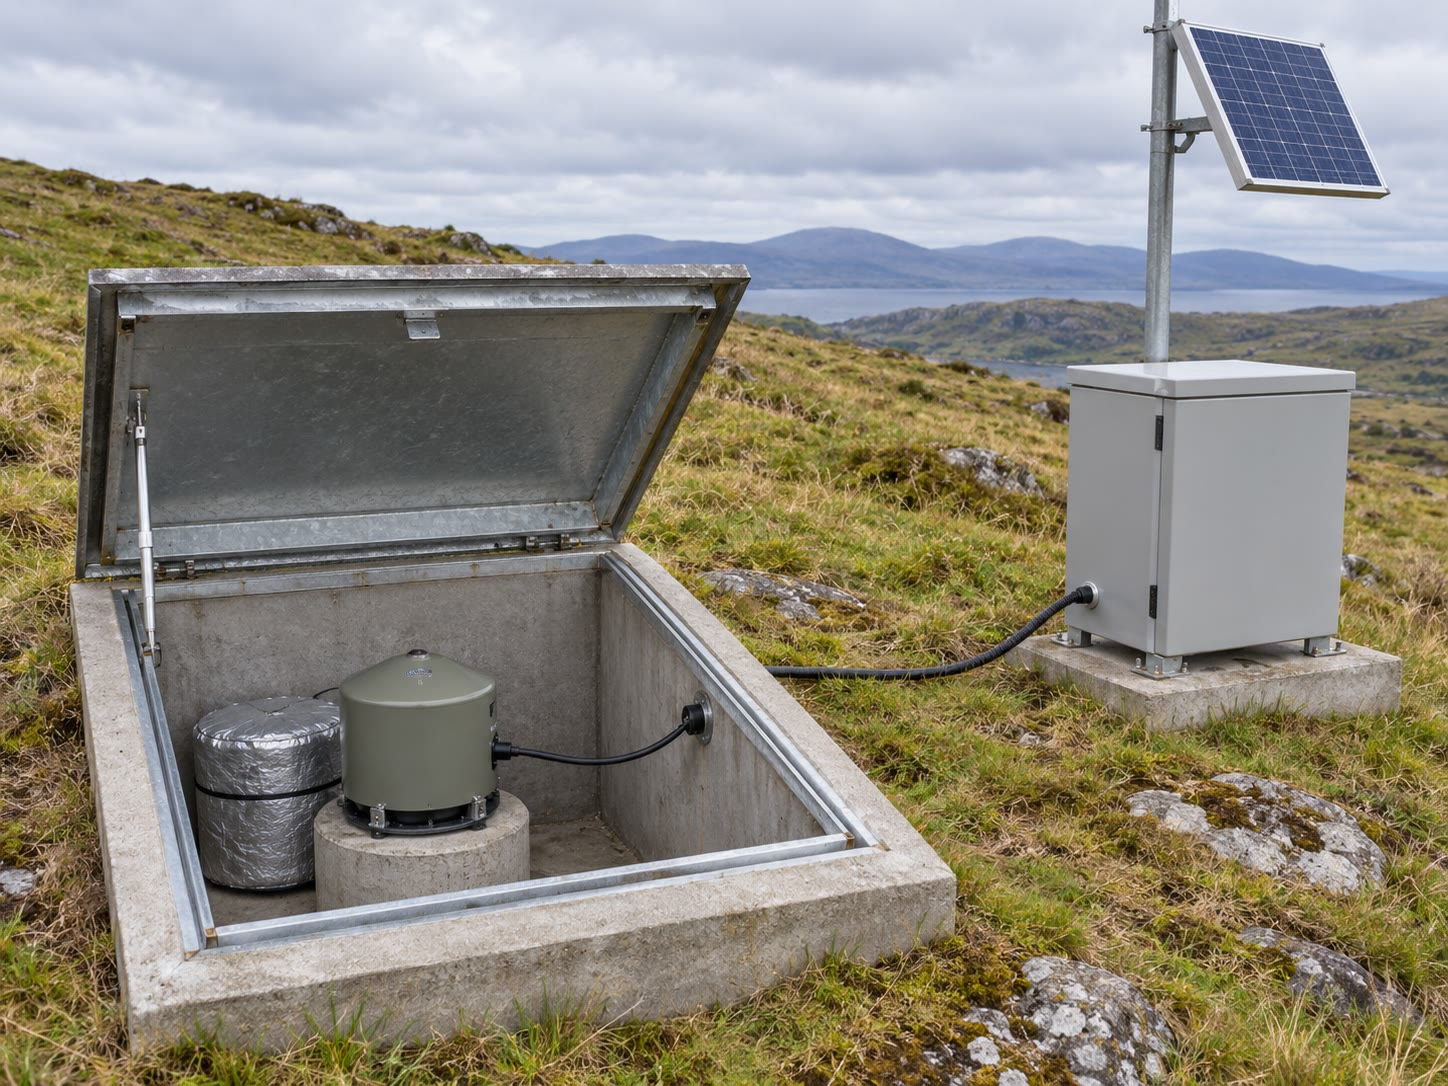
\includegraphics[width=\linewidth]{images/book5/ai/b3-seismic-vault.jpg}

{\scriptsize مقياس زلازل عريض النطاق على رصيفه في خزنة المحطة
(رسم توضيحي مولَّد بالذكاء الاصطناعي).}
\end{minipage}
\end{inthefield}

\section{التمارين}

\begin{exercise}[$\star$]\label{exo:b3:seismology-imaging:1}
يغادر شعاعُ P السطحَ ($R = \qty{6371}{km}$، $v_0 = \qty{5.80}{km.s^{-1}}$)
\omterm{def:b3:seismology-imaging:ray-parameter}{بمعامل الشعاع} $p = \qty{500}{s.rad^{-1}}$. (أ) احسب
زاوية انطلاقه. (ب) يعطي PREM سرعات P تبلغ \qty{11.066}{km.s^{-1}} عند عمق \qty{771}{km}
و\qty{11.245}{km.s^{-1}} عند \qty{871}{km}. احسب $r/v$ عند العمقين، ثم
أوجد عمق انعطاف الشعاع بالاستيفاء الخطّي.
% ledger: ak135:crust, data:prem
\end{exercise}

\begin{exercise}[$\star$]\label{exo:b3:seismology-imaging:2}
أزمنة P المحسوبة عبر PREM في هذا الفصل هي \qty{369.6}{s} عند \ang{30}
و\qty{455.5}{s} عند \ang{40}. (أ) قدّر ميل منحنى زمن الانتقال
بينهما، بوحدة \unit{s} لكلّ درجة وبوحدة \unit{s.rad^{-1}}. (ب) استنتج
السرعة الظاهرية لجبهة الموجة على طول السطح، بوحدة
\unit{km.s^{-1}}. (ج) ما سرعة P عند \omterm{def:b3:seismology-imaging:ray-parameter}{نقطة انعطاف الشعاع}
الواصل عند \ang{35}، إذا كان ينعطف عند نصف القطر \qty{5450}{km}؟
\end{exercise}

\begin{exercise}[$\star$]\label{exo:b3:seismology-imaging:3}
في نموذج \omterm{def:b3:seismology-imaging:surface-waves}{موجة لوف} لهذا الفصل، للطبقة $\beta_1 =
\qty{3.5}{km.s^{-1}}$، $\rho_1 = \qty{2700}{kg.m^{-3}}$ ونصف الفضاء
$\beta_2 = \qty{4.5}{km.s^{-1}}$، $\rho_2 = \qty{3300}{kg.m^{-3}}$.
(أ) احسب معاملَي القصّ. (ب) عند \qty{20}{s} تكون سرعة الطور
\qty{3.79}{km.s^{-1}}: احسب طول الموجة وقارنه مع الطبقة
سُمكها \qty{35}{km}. (ج) مع سرعتَي الزمرة \qty{3.384}{km.s^{-1}} عند
\qty{20}{s} و\qty{4.333}{km.s^{-1}} عند \qty{100}{s}، بكم دقيقةً تصل
الموجات \mbox{\textdir TLT 20-s} بعد الموجات \mbox{\textdir TLT 100-s} إلى محطة تبعد \qty{4000}{km}؟
\end{exercise}

\begin{exercise}[$\star$]\label{exo:b3:seismology-imaging:4}
الأدوار المرصودة للنمطين ${}_0S_2$ و${}_0T_2$ هي \qty{53.89}{min}
و\qty{44.01}{min}. (أ) احسب ترددَيهما بوحدة \unit{mHz}. (ب) كم
ذبذبةً من كلٍّ منهما تُنجزها الأرض في اليوم؟ (ج) لا يمكن فصل قمّتين طيفيّتين
إلا إذا دام التسجيل على الأقلّ مقلوب
فرق ترددَيهما. كم ينبغي أن يكون طول التسجيل لفصل هذين النمطين؟
% ledger: seis5:modes-S, seis5:modes-T
\end{exercise}

\begin{exercise}[$\star\star$]\label{exo:b3:seismology-imaging:5}
في كرةٍ نصف قطرها $R$ وسرعةٍ منتظمةٍ $v$، تكون الأشعة أوتارًا مستقيمة.
(أ) بيّن أنّ الشعاع الواصل إلى $\Delta$ زمنُ انتقاله
$T = 2R\sin(\Delta/2)/v$. (ب) مع $R = \qty{6371}{km}$
و$v = \qty{10.0}{km.s^{-1}}$، احسب $T$ عند \ang{30} و\ang{90}، وقارِنه
بأزمنة PREM، \qty{369.6}{s} و\qty{779.7}{s}. (ج) فسّر لماذا
الكرةُ المنتظمة أسرعُ من اللازم عند \ang{30} وأبطأُ من اللازم عند \ang{90}.
\end{exercise}

\begin{exercise}[$\star\star$]\label{exo:b3:seismology-imaging:6}
في جسم بواسون ($\lambda = \mu$، أي $\alpha^2 = 3\beta^2$) تُحقِّق سرعةُ \omterm{def:b3:seismology-imaging:surface-waves}{موجة رايلي}
$c$ المعادلةَ الآتية، مع $\xi = c^2/\beta^2$،
$(2 - \xi)^2 = 4\sqrt{1 - \xi/3}\,\sqrt{1 - \xi}$. (أ) ربِّعها وبيّن
أنّ الجذور تحقّق $(\xi - 4)(3\xi^2 - 12\xi + 8) = 0$. (ب) بيّن أنّ
الجذر الوحيد الذي يُحقّق $0 < \xi < 1$ هو $\xi = 2 - 2/\sqrt3$، واحسب $c/\beta$.
(ج) في القشرة العليا من النموذج ak135، $\beta = \qty{3.46}{km.s^{-1}}$: احسب
سرعةَ رايلي وتأخّرَ \omterm{def:b3:seismology-imaging:surface-waves}{موجة رايلي} خلف الموجة S عند
\qty{1000}{km}.
% ledger: ak135:crust
\end{exercise}

\begin{exercise}[$\star\star$]\label{exo:b3:seismology-imaging:7}
أزمنة وصول موجة الرأس عند أربع محطات من خطّ انكسار، على أبعاد 50، 100، 150
و\qty{200}{km} من نقطة الإطلاق، هي 9.0، 15.3، 21.5 و\qty{27.9}{s}، بأخطاء
0.1، 0.1، 0.2 و\qty{0.2}{s}. أجرِ ملاءمةً $T = a + bx$ بطريقة
المربعات الصغرى الموزونة: اكتب $\mathsf G$ و$\mathsf C_d$، وكوِّن المعادلات الطبيعية،
وأعطِ $a$، $b$، وأخطاءهما المعيارية، والسرعة $1/b$ مع خطئها،
وأدنى $\chi^2$. هل الملاءمة مقبولة؟
\end{exercise}

\begin{exercise}[$\star\star$]\label{exo:b3:seismology-imaging:8}
يعبر شعاعٌ واحد خليّتين، طولاهما \qty{30}{km} و\qty{40}{km}،
وله باقٍ قدره \qty{0.50}{s}. (أ) لماذا يكون $\mathsf N = \mathsf G^{\mathsf T}
\mathsf G$ منفردة؟ (ب) من بين النماذج التي تطابق الباقي تمامًا، النموذجُ
الذي له أصغر نظيم هو $\mathbf m = \mathsf G^{\mathsf T}(\mathsf G\mathsf
G^{\mathsf T})^{-1}\mathbf d$: احسبه. (ج) احسب المصفوفة
$\mathsf R = \mathsf G^{\mathsf T}(\mathsf G\mathsf G^{\mathsf T})^{-1}\mathsf G$
وأثرها. (د) إذا كان الشذوذ الحقيقي \qty{0.01}{s.km^{-1}} في الخلية
الأولى وحدها، فما الذي يُستعاد؟
\end{exercise}

\begin{exercise}[$\star\star$]\label{exo:b3:seismology-imaging:9}
منطقةٌ من اللوح المندس في الوشاح أسرع من محيطها بنسبة \qty{3}{\percent}،
حيث $v = \qty{9.0}{km.s^{-1}}$. (أ) احسب باقي شعاع يعبر
\qty{200}{km} منه رأسيًّا، حسب \cref{prop:b3:seismology-imaging:linear}،
وبدقّة تامّة. (ب) وبالمثل لشعاع يعبر سُمكًا قدره \qty{100}{km} منه بزاوية
\ang{40} عن العمودي على اللوح المندس. (ج) ما الخطأ النسبي في
التقريب الخطّي؟
\end{exercise}

\begin{exercise}[$\star\star\star$]\label{exo:b3:seismology-imaging:10}
في \cref{thm:b3:seismology-imaging:love}، توجد توافقية من الرتبة $n$ فقط
عند دورات قصيرة بما يكفي. (أ) بيّن أنّه عند تردّد القطع تكون سرعة طوره
$\beta_2$ و$kHq_1 = n\pi$. (ب) استنتج التردّد الزاوي للقطع
$\omega_n = n\pi\beta_1\beta_2/\bigl(H\sqrt{\beta_2^2 - \beta_1^2}\bigr)$.
(ج) احسب دور القطع للتوافقية الأولى لنموذج الفصل
($H = \qty{35}{km}$، $\beta_1 = 3.5$، $\beta_2 = \qty{4.5}{km.s^{-1}}$).
(د) بيّن أنّ النمط الأساسي لا يملك قطعًا، وأنّ سرعة طوره
تؤول إلى $\beta_1$ عند الدورات القصيرة.
\end{exercise}

\begin{exercise}[$\star\star\star$]\label{exo:b3:seismology-imaging:11}
خذ الشعاع من التمرين 8، مع خطأ معطيات يساوي الواحد. (أ) بيّن أنّه، من أجل أيّ
$\varepsilon > 0$، $(\mathsf G^{\mathsf T}\mathsf G + \varepsilon^2\mathsf
I)^{-1}\mathsf G^{\mathsf T} = \mathsf G^{\mathsf T}(\mathsf G\mathsf
G^{\mathsf T} + \varepsilon^2\mathsf I)^{-1}$. (ب) استنتج مصفوفة
الاستبانة المخمَّدة $\mathsf R_\varepsilon = \mathsf G^{\mathsf T}\mathsf G/(\|\mathbf g\|^2 +
\varepsilon^2)$، حيث $\mathbf g = (30, 40)$، وأثرها. (ج) احسب
الأثر وباقي المعطيات من أجل $\varepsilon^2 = 0$، 2500 و\num{10000}
(بالوحدة \unit{km^2}). صِف المقايضة.
\end{exercise}

\begin{exercise}[$\star\star\star$]\label{exo:b3:seismology-imaging:12}
في الكرة المتجانسة من التمرين 5: (أ) بيّن
حسب \cref{thm:b3:seismology-imaging:benndorf} أنّ $p(\Delta) = (R/v)\cos(\Delta/2)$،
وتحقّق من ذلك بمقارنته بتعريف $p$ (زاوية الإقلاع لوتر).
(ب) بيّن أنّ الشعاع الواصل إلى $\Delta_1$ ينعطف عند $r_1 = R\cos(\Delta_1/2)$.
(ج) بقبول أنّ $\int_0^{\Delta_1}\operatorname{arccosh}\bigl(\cos(\Delta/2)
/\cos(\Delta_1/2)\bigr)\,\mathrm d\Delta = \pi\ln\bigl(1/\cos(\Delta_1/2)\bigr)$،
بيّن أنّ صيغة \omterm{prop:b3:seismology-imaging:herglotz}{انعكاس هيرغلوتس--فيشرت} تُعيد $r_1$ والسرعة $v$.
\end{exercise}

\section{مسألة: اللوح المندس تحت المحطة K}

\begin{problem}[{مسألة نهاية الأسبوع --- أشعّة وموجات لوف وتصوير مقطعي صغير
تحت محطة مُتخيَّلة}]
\label{pb:b3:seismology-imaging:1}
% values: calc/ch01.py (invented station and models; Love-wave model as in the chapter)
تقع المحطة K على قارّة فوق منطقة اندساس. تستعمل هذه المسألة
سجلّاتها بثلاث طرق: أشعّة في قشرتها، وتشتّت موجات لوف عبرها،
وتصويرًا مقطعيًّا صغيرًا للوشاح تحتها.

\medskip
\noindent\textbf{الجزء الأول --- الأشعّة في تدرّج.} على مسافات قصيرة بما يكفي لإهمال
انحناء الأرض، تزداد سرعة الموجة P تحت K خطّيًّا مع العمق،
$v(z) = v_0 + gz$، مع $v_0 = \qty{5.0}{km.s^{-1}}$
و$g = \qty{0.05}{s^{-1}}$ ($z$ بالكيلومتر).
\begin{enumerate}
  \item في الطبقات المستوية، يُبقي قانون سنل $p = \sin i/v$ ثابتًا. ينطلق شعاع
        من K حيث $\sin i_0 = 0.8$: احسب $i_0$ و$p$.
  \item عند أيّ عمق ينعطف، وما السرعة هناك؟
  \item بيّن أنّ $\mathrm di/\mathrm ds = pg$ على طول الشعاع، فيكون قوسًا
        من دائرة؛ أعطِ نصف قطرها وعمق مركزها.
  \item احسب المسافة الأفقية $X$ التي يعود عندها الشعاع إلى
        السطح.
  \item بيّن أنّ $\mathrm dT = \mathrm di/(g\sin i)$ واحسب زمن
        الانتقال $T$ بدقّة.
  \item احسب $X$ و$T$ من أجل $p = \qty{0.15}{s.km^{-1}}$، وتحقّق من أنّ
        $\Delta T/\Delta X$ بين الشعاعين يقع بين قيمتي
        $p$.
\end{enumerate}

\noindent\textbf{الجزء الثاني --- موجات لوف والقشرة.} القشرة تحت K طبقةٌ
ذات سرعة S $\beta_1 = \qty{3.5}{km.s^{-1}}$ وكثافة
$\rho_1 = \qty{2.7}{g.cm^{-3}}$ فوق وشاحٍ ذي سرعة S $\beta_2 =
\qty{4.5}{km.s^{-1}}$، $\rho_2 = \qty{3.3}{g.cm^{-3}}$؛ سُمكها $H$
مجهولٌ. بين K ومحطة مجاورة تُقاس سرعة طور \omterm{def:b3:seismology-imaging:surface-waves}{موجة لوف}
فتبلغ \qty{3.99}{km.s^{-1}} عند \qty{25}{s} و\qty{4.25}{km.s^{-1}} عند
\qty{40}{s}.
\begin{enumerate}[resume]
  \item احسب $\mu_1$ و$\mu_2$ بالوحدة \unit{GPa}.
  \item عند \qty{25}{s}، احسب $k$، $q_1$ و$q_2$.
  \item حلّ معادلة التشتّت للنمط الأساسي من أجل $H$.
  \item أعِد الحساب نفسه عند \qty{40}{s}. هل النتيجتان متّسقتان؟
  \item قدّر سرعة الزمرة بين الدورين بالصيغة
        $\Delta\omega/\Delta k$، وقارنها بسرعات الطور.
  \item احسب طول الموجة عند كلّ دور، واشرح لماذا يستشعر كلٌّ
        من الدورين القشرةَ والجزءَ الأعلى من الوشاح بنسب
        مختلفة.
\end{enumerate}

\noindent\textbf{الجزء الثالث --- تصوير مقطعي في أربع خلايا.} تحت K، كتلةٌ من
الوشاح بأبعاد \qty{200}{km} × \qty{200}{km} في مقطع رأسي، مقسَّمةٌ إلى أربع
خلايا مربّعة ضلعها \qty{100}{km}: 1 (أعلى اليسار)، 2 (أعلى اليمين)، 3 (أسفل اليسار)
و4 (أسفل اليمين)؛ يقع الخندق والمحيط إلى اليسار. السرعة المرجعية $v_0 = \qty{8.0}{km.s^{-1}}$. في
تجربة مثالية تعبره ستّة أشعّة مستقيمة: A على طول الصفّ العلوي (الخليتين 1
و2)، B على طول الصفّ السفلي (3 و4)، C على طول العمود الأيسر (1 و3)، D
على طول العمود الأيمن (2 و4)، E على طول القطر المارّ بالخليتين 1 و4، F على طول
القطر المارّ بالخليتين 2 و3. وبواقيها هي:
\begin{center}
\small
\begin{tabular}{lcccccc}
\hline
الشعاع & A & B & C & D & E & F \\
\mbox{\textdir TLT $\delta t$ (\unit{s})} & $0.16$ & $-0.48$ & $-0.36$ & $0.11$ & $-0.15$ & $-0.27$ \\
الخطأ $\sigma$ \babelsublr{(\unit{s})} & 0.05 & 0.05 & 0.05 & 0.05 & 0.10 & 0.10 \\
\hline
\end{tabular}
\end{center}
خذ النموذج $\mathbf m$ على أنّه اضطرابات البطء للخلايا
بوحدة \unit{ms.km^{-1}} ($\qty{1}{ms.km^{-1}} = \qty{e-3}{s.km^{-1}}$)، بحيث تكون
عناصر $\mathsf G$ هي أطوال الأشعّة بوحدة \unit{km} مقسومةً على 1000.
\begin{enumerate}[resume]
  \item اكتب $\mathsf G$، وهي مصفوفة $6\times4$.
  \item بيّن أنّ $\mathsf N = \mathsf G^{\mathsf T}\mathsf C_d^{-1}\mathsf G$
        لها الصفوف $(10, 4, 4, 2)$، $(4, 10, 2, 4)$، $(4, 2, 10, 4)$،
        $(2, 4, 4, 10)$.
  \item احسب $\mathbf b = \mathsf G^{\mathsf T}\mathsf C_d^{-1}\mathbf d$.
  \item تحقّق من أنّ $(1,1,1,1)$، $(1,-1,-1,1)$، $(1,1,-1,-1)$ و$(1,-1,1,-1)$
        متجهات ذاتية للمصفوفة $\mathsf N$، بالقيم الذاتية 20، 4، 8 و8،
        واستنتج أنّ $\mathsf N^{-1}$ لها الصفوف $(11, -4, -4, 1)/80$،
        $(-4, 11, 1, -4)/80$، $(-4, 1, 11, -4)/80$ و$(1, -4, -4, 11)/80$.
  \item احسب \omterm{thm:b3:seismology-imaging:wls}{تقدير المربعات الصغرى الموزونة} $\hat{\mathbf m}$.
  \item حوّله إلى شذوذات نسبية للسرعة $\delta v/v_0$ بالنسبة المئوية.
  \item أعطِ الخطأ المعياري لكلّ خلية بوحدة \unit{ms.km^{-1}} وبالنسبة
        المئوية، والترابط بين الخليتين 1 و2، وبين الخليتين 1
        و4. فسّر إشاراتها.
  \item احسب بواقي الأشعّة الستّة بعد الملاءمة، وأدنى
        $\chi^2$. هل تتّسق مع الأخطاء المعطاة؟
\end{enumerate}

\noindent\textbf{الجزء الرابع --- التخميد والاستبانة واللوح المندس.}
\begin{enumerate}[resume]
  \item من أجل $\varepsilon^2 = 4$ (بوحدات $\mathsf N$)، أعطِ
        القيم الذاتية للمصفوفة $\mathsf R = (\mathsf N + 4\mathsf I)^{-1}\mathsf N$
        وبيّن أنّ $\mathsf R$ قطرها $2/3$، وأنّ المدخلات $1/12$
        بين الخلايا التي تتشارك شعاعَ صفٍّ أو عمودٍ، و$0$ بين الخليتين 1
        و4 وبين الخليتين 2 و3.
  \item احسب التقدير المخمَّد للخلية 3 وشذوذ سرعتها. لماذا يكون
        أصغر من غير المخمَّد؟
  \item النموذج المخمَّد له $\chi^2 = 15.8$ ونظيم قدره \qty{2.91}{ms.km^{-1}}؛
        وغير المخمَّد، $\chi^2 = 0.50$ و\qty{4.24}{ms.km^{-1}}. أيّهما
        يُستبقى، ولماذا لا تحتاج هذه المسألة إلى تخميد؟
  \item اقرأ الصفّ 3 من المصفوفة $\mathsf R$ المخمَّدة: مع أيّ خلايا يكون
        تقدير الخلية 3 مموَّهًا؟
  \item أيّ خلية سريعة وأيّها بطيئة؟ فسّر الخلية السريعة الواقعة تحت
        K وعلى جهة المحيط منها، بدلالة منطقة الاندساس.
  \item أعطِ شذوذ سرعة الموجة P لخلية اللوح المندس بالنسبة المئوية، مع
        خطئها المعياري.
\end{enumerate}
\end{problem}
